\documentclass[t]{beamer}

%\documentclass[handout, t]{beamer}
\setbeamertemplate{navigation symbols}{}
\usepackage{pstricks}
\usepackage{mathtools}
\usepackage{amsfonts}
\usepackage{mathrsfs}
\usepackage{amsmath}
\setbeamertemplate{navigation symbols}{}
\usepackage{bm}
\usepackage[UTF8]{ctex}
\usetheme{AnnArbor}
\usefonttheme{serif}
\useinnertheme{rounded}
\usecolortheme{dolphin}
\setbeamertemplate{blocks}[rounded][shadow=true]

\newcommand{\dif}{{\;\rm d}}
\usepackage{graphicx}
\usepackage{pgf}
\usepackage{tikz}
\usetikzlibrary{arrows, decorations.pathmorphing, backgrounds, positioning, fit, petri, automata}
\tikzset{>=stealth}

\usepackage{setspace}
\setmainfont{Times New Roman}
\setCJKmainfont{Microsoft YaHei}
% \setCJKmainfont{苹方}   % 使用苹果MAC系统,请使用这个选项,并将上面的命令用%注释掉

\hypersetup{pdfpagemode=FullScreen}
\renewcommand{\Pr}{\mathbb{P}}
\usepackage{blkarray}


\setbeamercolor{block title}{bg=red!10!white}
\setbeamercolor{block body}{bg=gray!10!white}

\usepackage{multicol}
\newcommand{\E}{\mathbb{E}}
\newcommand{\EP}{\mathbb{E}^{\mathbb{P}}}
\newcommand{\EQ}{\mathbb{E}^{\mathbb{Q}}}
\newcommand{\Var}{{\rm Var}}
\newcommand{\Cov}{{\rm Cov}}


\begin{document}
\fontsize{11}{18}\selectfont


\CTEXindent



  \title{第七章~~连续时间下的期权定价}
\author{金融数学}
\date{中国人民大学出版社}
  \begin{frame}
    \maketitle
  \end{frame}

\begin{frame}{简介}
	自从期权交易产生以来,人们就一直致力于对期权定价问题的探讨。
	1973年美国芝加哥大学教授费希尔·布莱克(Fischer Black, 1938---1995)和迈伦·斯科尔斯(Myron  Scholes, 1941---\,)发表了《期权定价与公司负债》一文,提出了有史以来的第一个期权定价模型,在学术界和实务界引起了强烈的反响。
	
	在布莱克和斯科尔斯研究的基础上,罗伯特·默顿(Robert Merton, 1944---\,)独立地使用随机微积分的相关方法对期权定价问题进行了研究,于同年在《贝尔经济与管理科学杂志》上发表了名为《期权的理性定价理论》的论文。
\end{frame}

\begin{frame}{三位学者}
	这两篇论文奠定了期权定价的理论基础。他们所提出的期权定价模型称作布莱克-斯科尔斯(Black-Scholes)期权定价模型(后文简称为B-S模型)。
	由于这三位学者的突出贡献,最终默顿和斯科尔斯于1997年获得诺贝尔经济学奖。
\begin{center}
\begin{tabular}{ccc}
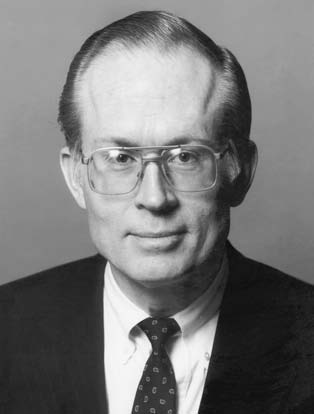
\includegraphics[height=0.4\textheight]{fig/black.jpg}
& \includegraphics[height=0.4\textheight]{fig/Scholes.jpg}& \includegraphics[height=0.4\textheight]{fig/Merton.jpg}\\
Fischer Black & Myron Scholes & Robert C. Merton
\end{tabular}
\end{center}

\end{frame}




\begin{frame}{本章内容}
\tableofcontents

\end{frame}

\section{期权的价格分析}
\begin{frame}{看涨期权的价格分析}
看涨期权(call option)的买方在未来具有按照行权价买入标的资产的权利。
假设$S$表示标的资产在未来期权到期时的市价;$K$表示期权的行权价。因此对于看涨期权买方而言,其未来到期时的回报数额(payoff)如下:
\begin{equation*}
V_C=(S-K)^+=\max[S-K,0]=\begin{cases}
S-K,& S\ge K\\
0,& S<K
\end{cases}
\end{equation*}
对于看涨期权而言,只有当$S\ge K$时,期权才有必要行权,因此行权后的回报数额即为标的资产高价与行权价之差;否则期权将放弃行权,相应的回报数额为零。

\end{frame}

\begin{frame}{看涨期权的价格分析(cont.)}
\begin{equation*}
V_C=(S-K)^+=\max[S-K,0]=\begin{cases}
S-K,& S\ge K\\
0,& S<K
\end{cases}
\end{equation*}
\begin{itemize}
\item 当$S=K$时,看涨期权是平值(in-the-money, ITM)期权;
\item 当$S>K$时,看涨期权是实值(at-the-money, ATM)期权;
\item 当$S<K$时,看涨期权是虚值(out-of-the-money, OTM)期权。
\item 对于看涨期权而言,实值期权的回报数额为正;虚值和平值期权的回报数额则为零。
\end{itemize}

\end{frame}

\begin{frame}{看跌期权的价格分析}
看跌期权(put option)的买方在未来具有按照行权价卖出标的资产的权利。因此其未来到期时的回报数额如下:
\begin{equation*}
V_P=(K-S)^+=\max[K-S,0]=\begin{cases}
0,& S> K\\
K-S,& S\le K
\end{cases}
\end{equation*}
类似地,当$S=K$时,看跌期权是平值期权;当$S<K$时,看跌期权是实值期权;当$S>K$时,看跌期权是虚值
期权。
\end{frame}

\begin{frame}{总结:期权的回报数额与实虚值对应关系}
\begin{center}
\begin{tabular}{c|cc|cc}
\hline
& 看涨期权&回报额 &看跌期权&回报额 \\
\hline
实值 & $S>K$&$S-K$  & $S<K$&$K-S$ \\
虚值 & $S<K$&0  & $S>K$&0\\
平值 & $S=K$&0  & $S=K$&0\\
\hline
\end{tabular}
\end{center}
\end{frame}


\section{期权与标的资产的对冲}

\begin{frame}{B-S模型与几何布朗运动}
在B-S模型当中,假设期权标的资产价格的演化服从几何布朗运动,即:
\begin{equation*}
\dif S(t)=\mu S(t)\dif t+\sigma S(t)\dif W(t)
\end{equation*}
其中:$\mu$和$\sigma$均是常数,分别是标的资产$S$的漂移率和波动率;$W(t)$是标准布朗运动。

由于期权是由标的资产衍生而来,因此其价格变动受到标的资产价格的影响。记期权的价格为$f[S(t)]$。
\end{frame}




\begin{frame}{期权价格的随机偏微分方程(SPDE)}
根据伊藤引理可得:
\begin{equation*}
\begin{split}
\dif f&=\frac{\partial f}{\partial t}\dif t+\frac{\partial f}{\partial S}\dif S+\frac{1}{2}\frac{\partial^2 f}{\partial S^2}[\dif S]^2\\
&=\left[\frac{\partial f}{\partial t}+\mu S\frac{\partial f}{\partial S}+\frac{1}{2}\sigma^2S^2\frac{\partial^2 f}{\partial S^2} \right]\dif t+\sigma S\frac{\partial f}{\partial S}\dif W(t)
\end{split}
\end{equation*}

\begin{block}{}
在B-S模型的原始文献中,采用将期权与标的资产构成的组合进行对冲的方式,并基于无套利原理,最终得到求解期权价格的方程。
\end{block}
\end{frame}

\begin{frame}{资产组合的构建}
假设构造的组合中包含了一份期权,以及$\Delta$份标的资产,并将该组合的总价值记为$\Pi$,因此:
\begin{equation*}
\Pi=f+\Delta S
\end{equation*}
于是该资产组合的价值变动为:
\begin{equation*}
\dif \Pi=\dif f+\Delta \dif S
\end{equation*}
将下式代入上式
\[\begin{cases}
\vspace{1ex}\dif S(t)=\mu S(t)\dif t+\sigma S(t)\dif W(t)\\
\dif f=\left[\dfrac{\partial f}{\partial t}+\mu S\dfrac{\partial f}{\partial S}+\dfrac{1}{2}\sigma^2S^2\dfrac{\partial^2 f}{\partial S^2} \right]\dif t+\sigma S\dfrac{\partial f}{\partial S}\dif W(t)
\end{cases}\]
\end{frame}

\begin{frame}{资产组合的构建(cont.)}
\begin{equation*}
\dif \Pi=\left[\frac{\partial f}{\partial t}+\mu S\frac{\partial f}{\partial S}+\frac{1}{2}\sigma^2S^2\frac{\partial^2 f}{\partial S^2}+\Delta\mu S \right]\dif t+\left[\sigma S\frac{\partial f}{\partial S}+\Delta\sigma S\right]\dif W(t)
\end{equation*}

接下来,令上式中的$\dif W(t)$项取值为零,则意味着:
\[\Delta=-\frac{\partial f}{\partial S}  \]
此时,组合$\Pi$的价格变动不受随机因素的影响,对应地:
\begin{equation*}
\dif \Pi=\left[\frac{\partial f}{\partial t}+\frac{1}{2}\sigma^2S^2\frac{\partial^2 f}{\partial S^2} \right]\dif t
\end{equation*}

{\color{red}投资组合的价值变动仅与时间$t$的变动有关,该组合已经消除了随机因素带
来的不确定性。}
\end{frame}

\begin{frame}{无风险资产组合}
根据无套利定价原理,该投资组合的收益率应该等于无风险利率$r$。因此在连续复利计息下,下式成立:
\[\Pi(T)=\Pi(t)e^{r(T-t)} \]
与之对应的微分方程如下:
\begin{equation*}
\dif \Pi=r\Pi \dif t
\end{equation*}
与$\dif \Pi=\left[\frac{\partial f}{\partial t}+\frac{1}{2}\sigma^2S^2\frac{\partial^2 f}{\partial S^2} \right]\dif t$联立,可得:
\[\left[\frac{\partial f}{\partial t}+\frac{1}{2}\sigma^2S^2\frac{\partial^2 f}{\partial S^2} \right]\dif t=r\left[f-\frac{\partial f}{\partial S} S\right]\dif t \]
\end{frame}

\begin{frame}{B-S偏微分方程}
\[\left[\frac{\partial f}{\partial t}+\frac{1}{2}\sigma^2S^2\frac{\partial^2 f}{\partial S^2} \right]\dif t=r\left[f-\frac{\partial f}{\partial S} S\right]\dif t \]
整理可得:
\begin{equation*}
\frac{\partial f}{\partial t}+rS\frac{\partial f}{\partial S}+\frac{1}{2}\sigma^2S^2\frac{\partial^2 f}{\partial S^2} =rf
\end{equation*}
上式就是著名的B-S偏微分方程(Partial Differential Equation, PDE) 。
求解该方程,最终得到的$f[S(t)]$ 就是期权的合理价格。
\end{frame}

\begin{frame}{B-S偏微分方程}
\[\frac{\partial f}{\partial t}+rS\frac{\partial f}{\partial S}+\frac{1}{2}\sigma^2S^2\frac{\partial^2 f}{\partial S^2} =rf\]
这个偏微分方程有很多解,为此需要
添加必要的边界条件(Boundary Condition)才有可能得到唯一的解。

\begin{itemize}
\item 对于到期时间为$T$的{\color{blue}欧式看涨期权}来说,该边界条件是$f[S(t)]=\max\big[S(T)-K,0\big]$;
\item 对于{\color{red}欧式看跌期权}来说,边界条件则为
$f[S(t)]=\max\big[K-S(T),0\big]$。
\end{itemize}
\end{frame}

\begin{frame}{倒向偏微分方程}
	这个偏微分方程的边界条件与自然科学领域
常见问题的边界条件有所区别。从严格意义上说,B-S偏微分方程是一种倒向偏微分方程(backward PDE)。

\begin{center}\small
	\begin{tikzpicture}[>=stealth, thick, scale=.8]

		\draw[->](0,0)--(9,0);
		\foreach \x in {0, 3, 8}
		{\draw(\x,-.1)--(\x,.1);
		}
		
		\node [below] at (0,-0.1) {$0$};
		\node [below] at (3,-0.1) {$t$};
		\node [below] at (8,-0.1) {$T$};
		\node [above] at (9,0.1) {时间};
		
		\node  at (0,.75) {初始条件已知};
		\node  at (3,.75) {?};
		\node  at (8,.75) {?};
		\node  at (1.5,.75) {$\to$};
		\node  at (5.5,.75) {$\to\quad \cdots\quad \to$};
		\node  at (-3,.75) {物理学领域:};
		
		
		\node  at (0,-1) {?};
		\node  at (3,-1) {?};
		\node at (8,-1) {终值条件已知};
		\node  at (1.5,-1) {$\leftarrow$};
		\node  at (5.5,-1) {$\leftarrow\quad \cdots\quad \leftarrow$};
		\node  at (-3,-1) {衍生品定价领域:};
		\end{tikzpicture}
\end{center}

\end{frame}





\section{期权的风险中性定价法}
\begin{frame}{风险中性定价法}
风险中性概率测度$\mathbb{Q}$下,资产价格的贴现值是鞅。基于这一结论,我们使用风险中性方法对欧式看涨期权进行定价。

对于服从几何布朗运动的标的资产而言,在测度$\mathbb{Q}$下,其价格演化的随机微分方程当中的漂移项即为无风险利率$r$,因此:
\begin{equation*}
\dif S(t)=rS(t)\dif t+\sigma S(t)\dif \widetilde{W}(t)
\end{equation*}
其中:$\widetilde{W}(t)$是测度$\mathbb{Q}$下的标准布朗运动。根据伊藤引理可得:
\begin{equation*}
\begin{split}
S(t)&=S(0)\exp\left[\left( r-\frac{1}{2}\sigma^2\right)  t+\sigma \widetilde{W}(t)\right] \\
&=S(0)\exp\left[\left( r-\frac{1}{2}\sigma^2\right)  t+\sigma \sqrt{t}Z\right]
\end{split}
\end{equation*}
其中:$Z\sim \mathcal{N}(0,1)$。
\end{frame}

\subsection{欧式期权的定价}
\begin{frame}{欧式看涨期权的定价}
	对于欧式看涨期权而言,其未来到期时的回报数额为$\max[S(T)-K,0]$,也常常简写为$[S(T)-K]^+$,根据风险中性测度的性质,可得:
\begin{equation*}
V(0)=e^{-rT}\EQ[V(T)|S(0)=S]=e^{-rT}\EQ\left[(S(T)-K)^+\Big|S(0)=S\right]
\end{equation*}
于是:
\[\begin{split}
V(0)&=e^{-rT} \int^{\infty}_{-\infty} \left( S\exp\left[\left( r-\frac{1}{2}\sigma^2\right)  T+\sigma z \sqrt{T}\right]-K\right) ^+ f_Z(z)\dif z\\
&=e^{-rT} \int^{\infty}_{\color{red}z_0} \left( S\exp\left[\left( r-\frac{1}{2}\sigma^2\right)  T+\sigma z \sqrt{T}\right]-K\right) f_Z(z)\dif z\\
\end{split} \]
\end{frame}

\begin{frame}{欧式看涨期权的定价(cont.)}
$f_Z(z)$是标准正态分布的概率密度函数,即:
\[f_Z(z)=\frac{1}{\sqrt{2\pi}}\exp\left[-\frac{z^2}{2}\right] \]
$z_0$计算过程如下:
\[S\exp\left[\left( r-\frac{1}{2}\sigma^2\right)  T+\sigma z_0 \sqrt{T}\right]=K\;\Rightarrow \;
{\color{blue}z_0=\frac{\ln (K/S)-\left( r-\frac{1}{2}\sigma^2\right)  T}{\sigma\sqrt{T}}}
\]
\end{frame}

\begin{frame}{欧式看涨期权的定价(cont.)}
\[V(0)=e^{-rT} \int^{\infty}_{z_0} \left( S\exp\left[\left( r-\frac{1}{2}\sigma^2\right)  T+\sigma z \sqrt{T}\right]-K\right) f_Z(z)\dif z\]
$V(0)$可进一步拆分成两项:
\[\begin{split}
V(0)&=Se^{-rT} {\color{red}\int^{\infty}_{z_0}  \exp\left[\left( r-\frac{1}{2}\sigma^2\right)  T
+\sigma z \sqrt{T}\right]f_Z(z)\dif z}
-Ke^{-rT}{\color{blue}\int^{\infty}_{z_0}  f_Z(z)\dif z}\\
&=Se^{-rT} {\color{red}I_1}-Ke^{-rT}{\color{blue}N(-z_0)}
\end{split} \]
\end{frame}

\begin{frame}{$I_1=?$}
\[\begin{split}
I_1&=\int^{\infty}_{z_0} \exp\left[\left(r-\frac{1}{2}\sigma^2 \right) T+\sigma \sqrt{T} z\right]f_Z(z)\dif z\\
&=\int^{\infty}_{z_0} \exp\left[\left(r-\frac{1}{2}\sigma^2 \right) T+\sigma \sqrt{T} z\right]\frac{1}{\sqrt{2\pi}}\exp\left[-\frac{1}{2}z^2\right] \dif z\\
&=\frac{1}{\sqrt{2\pi}}\int^{\infty}_{z_0}\exp\left[-\frac{(z-\sigma\sqrt{T})^2}{2}\right]\exp\left[rT\right]\dif z\\
u=z-\sigma\sqrt{T} \to &={e^{rT}}\left\{\frac{1}{\sqrt{2\pi}}\int^{\infty}_{z_0-\sigma\sqrt{T}}\exp\left[-\frac{u^2}{2}\right]\dif u\right\}\\
&={e^{rT}}N(-z_0+\sigma\sqrt{T})
\end{split} \]
\end{frame}

\begin{frame}{欧式看涨期权的定价(cont.)}
最终:
\begin{equation*}
\begin{split}
V(0)&=SN\left(\frac{\ln(S/K)+(r+\frac{1}{2}\sigma^2)T}{\sigma\sqrt{T}} \right)-Ke^{-rT} N\left(\frac{\ln(S/K)+(r-\frac{1}{2}\sigma^2)T}{\sigma\sqrt{T}} \right) \\
&=SN(d_1)-Ke^{-rT}N(d_2)
\end{split}
\end{equation*}
其中:
\[d_1=\frac{\ln \left( S/K \right) +\left( r+\frac{1}{2}\sigma ^2 \right) T}{\sigma \sqrt{T}},\qquad d_2=\frac{\ln \left( S/K \right) +\left( r-\frac{1}{2}\sigma ^2 \right) T}{\sigma \sqrt{T}} \]
\end{frame}


\subsection{两类二元期权的定价}

\begin{frame}{一类二元期权}
对于看涨型二元期权而言,当未来标的资产价格超过行权价$K$时,投资者将得到1元的回报;否则将得不到任何回报。对于这样的期权,其未来 时刻的回报函数可以使用示性函数来表示,即:
\[{\bf 1}_{\{S(T)>K\}}=\begin{cases}
1,& S(T)>K\\
0,& S(T)\le K
\end{cases} \]
对此可以给出当前时刻期权的价格计算公式如下:
\[V(0)=e^{-rT}\EQ\left[{\bf 1}_{\{S(T)>K\}}|S(0)=S\right] \]
\end{frame}

\begin{frame}{一类二元期权(cont.)}
根据示性函数的性质,可得:
\begin{equation*}
\begin{split}
V(0)&=e^{-rT}\mathbb{Q}[S(T)>K|S(0)=S]\\
&=e^{-rT}\mathbb{Q}\left[S\exp\left[\left(r-\frac{1}{2}\sigma^2 \right) T+\sigma \widetilde{W}(T)\right]>K \right]\\
&=e^{-rT}\mathbb{Q}\left\{\widetilde{W}(T)>\frac{1}{\sigma}\left[\ln\left( \frac{K}{S}\right) -\left(r-\frac{1}{2}\sigma^2 \right) T\right] \right\}\\
&=e^{-rT}\mathbb{Q}\left\{Z>\frac{1}{\sigma\sqrt{T}}\left[\ln\left( \frac{K}{S}\right) -\left(r-\frac{1}{2}\sigma^2 \right) T\right] \right\}\\
&=e^{-rT}N\left(\frac{\ln\left( \frac{S}{K}\right) +\left(r-\frac{1}{2}\sigma^2 \right) T}{\sigma\sqrt{T}} \right)
\end{split}
\end{equation*}
因此:\begin{equation*}
V(0)=e^{-rT}N(d_2)
\end{equation*}
\end{frame}

\begin{frame}{二元期权的分类}
刚才所提到的二元期权,从严格意义上说,属于{\color{blue}或有现金形式(cash-or-nothing)}的二元期权品种,也就是期权到期时支付固定数额或者不支付任何金额。

实际上还有一类{\color{red}或有资产形式(asset-or-nothing)}的二元期权,即期权到期时支付标的资产或者不支付任何实物。

或有资产形式二元期权的看涨期权,当未来到期时,若标的资产价格$S(T)$大于行权价$X$时,则期权的买方将得到该标的资产,否则买方则一无所获。
因此这类期权的回报函数如下:
\[S(T){\bf 1}_{\{S(T)>K\}}=\begin{cases}
S(T),& S(T)>K\\
0,& S(T)\le K
\end{cases} \]
\end{frame}

\begin{frame}{或有资产形式的二元期权定价}
根据风险中性定价法,当前时刻期权的价格计算公式如下:
\[V(0)=e^{-rT}\EQ\left[S(T){\bf 1}_{\{S(T)>K\}}|S(0)=S\right] \]
根据示性函数的性质,可得:
\[\begin{split}
V(0)&=e^{-rT}\int^{\infty}_{-\infty} S\exp\left[\left(r-\frac{1}{2}\sigma^2 \right) T+\sigma \sqrt{T} z\right] {\bf 1}_{\{S(T)>K\}} f_Z(z)\dif z\\ 
&=e^{-rT}\int^{\infty}_{z_0} S\exp\left[\left(r-\frac{1}{2}\sigma^2 \right) T+\sigma \sqrt{T} z\right] f_Z(z)\dif z\\ 
\end{split} \]
其中:
\[z_0=\frac{\ln(K/S)-\left(r-\frac{1}{2}\sigma^2 \right) T}{\sigma \sqrt{T}}\]
\end{frame}

\begin{frame}{或有资产形式的二元期权定价(cont.)}
\[
V(0)=Se^{-rT}\int^{\infty}_{z_0} \exp\left[\left(r-\frac{1}{2}\sigma^2 \right) T+\sigma \sqrt{T} z\right]f_Z(z)\dif z=Se^{-rT}I_1
 \]
其中:
\[\begin{split}
I_1&=\int^{\infty}_{z_0} \exp\left[\left(r-\frac{1}{2}\sigma^2 \right) T+\sigma \sqrt{T} z\right]f_Z(z)\dif z\\
&=\int^{\infty}_{z_0} \exp\left[\left(r-\frac{1}{2}\sigma^2 \right) T+\sigma \sqrt{T} z\right]\frac{1}{\sqrt{2\pi}}\exp\left[-\frac{1}{2}z^2\right] \dif z\\
&=\frac{1}{\sqrt{2\pi}}\int^{\infty}_{z_0}\exp\left[-\frac{(z-\sigma\sqrt{T})^2}{2}\right]\exp\left[rT\right]\dif z\\
&={e^{rT}}N(-z_0+\sigma\sqrt{T})
\end{split} \]
\end{frame}

\begin{frame}{或有资产形式的二元期权定价(cont.)}
最终:
\begin{equation*}
\begin{split}
V(0)&=SN(-z_0+\sigma\sqrt{T})\\
&=SN\left(\frac{\ln(S/K)+(r+\frac{1}{2}\sigma^2)T}{\sigma\sqrt{T}} \right)\\&=SN(d_1) 
\end{split}
\end{equation*}
\end{frame}


\subsection{欧式看涨期权与二元期权的关系}
\begin{frame}{欧式看涨期权与二元期权的关系}\Large
\begin{center}
\begin{tabular}{cc}
\hline
期权种类 & 定价公式   \\
\hline
欧式看涨期权 &  $SN(d_1)-Ke^{-rT}N(d_2)$  \\
或有现金形式的看涨二元期权 &  $e^{-rT}N(d_2)$  \\
或有资产形式的看涨二元期权 &  $SN(d_1)$  \\
\hline
\end{tabular}
\end{center}

\begin{block}{}
对于普通的欧式看涨期权买方而言,其相当于{\color{red}买入}了一份或有资产形式的看涨二元期权,同时{\color{magenta}卖出}了$K$份或有现金形式的看涨二元期权的组合。
\end{block}
\end{frame}

\subsection{障碍期权的定价}



\begin{frame}{障碍期权的概念和分类}\small
	\begin{spacing}{1.3}
		障碍期权是指在期权的期限内,当标的资产价格达到某一水平时,既可以被启动也可以被取消的期权。
	
	在障碍期权中,除了行权价外,还增设了一个障碍价格。障碍期权总是比普通期权便宜。障碍期权的收益依赖于标的资产的价格在一段特定时间内是否达到一个特定水平。其与标准期权不同的是,在期权有效期内,当标的资产的价格达到某一水平时,期权就生效或失效。

	障碍期权一般分为两类,即敲出期权和敲入期权。敲出期权是指当标的资产价格达到一个特定障碍水平时,该期权作废。敲入期权是指只有当标的资产价格达到一个特定障碍水平时,该期权才有效。敲出期权既可向上敲出(up-and-out),也可向下敲出(down-and-out)。同样,敲入期权也既可向上敲入(up-and-in),又可向下敲入(down-and-in)。于是,障碍期权可分为四种。
	\end{spacing}
	

\end{frame}

\begin{frame}{障碍期权的敲入/敲出示意图}
	\centering
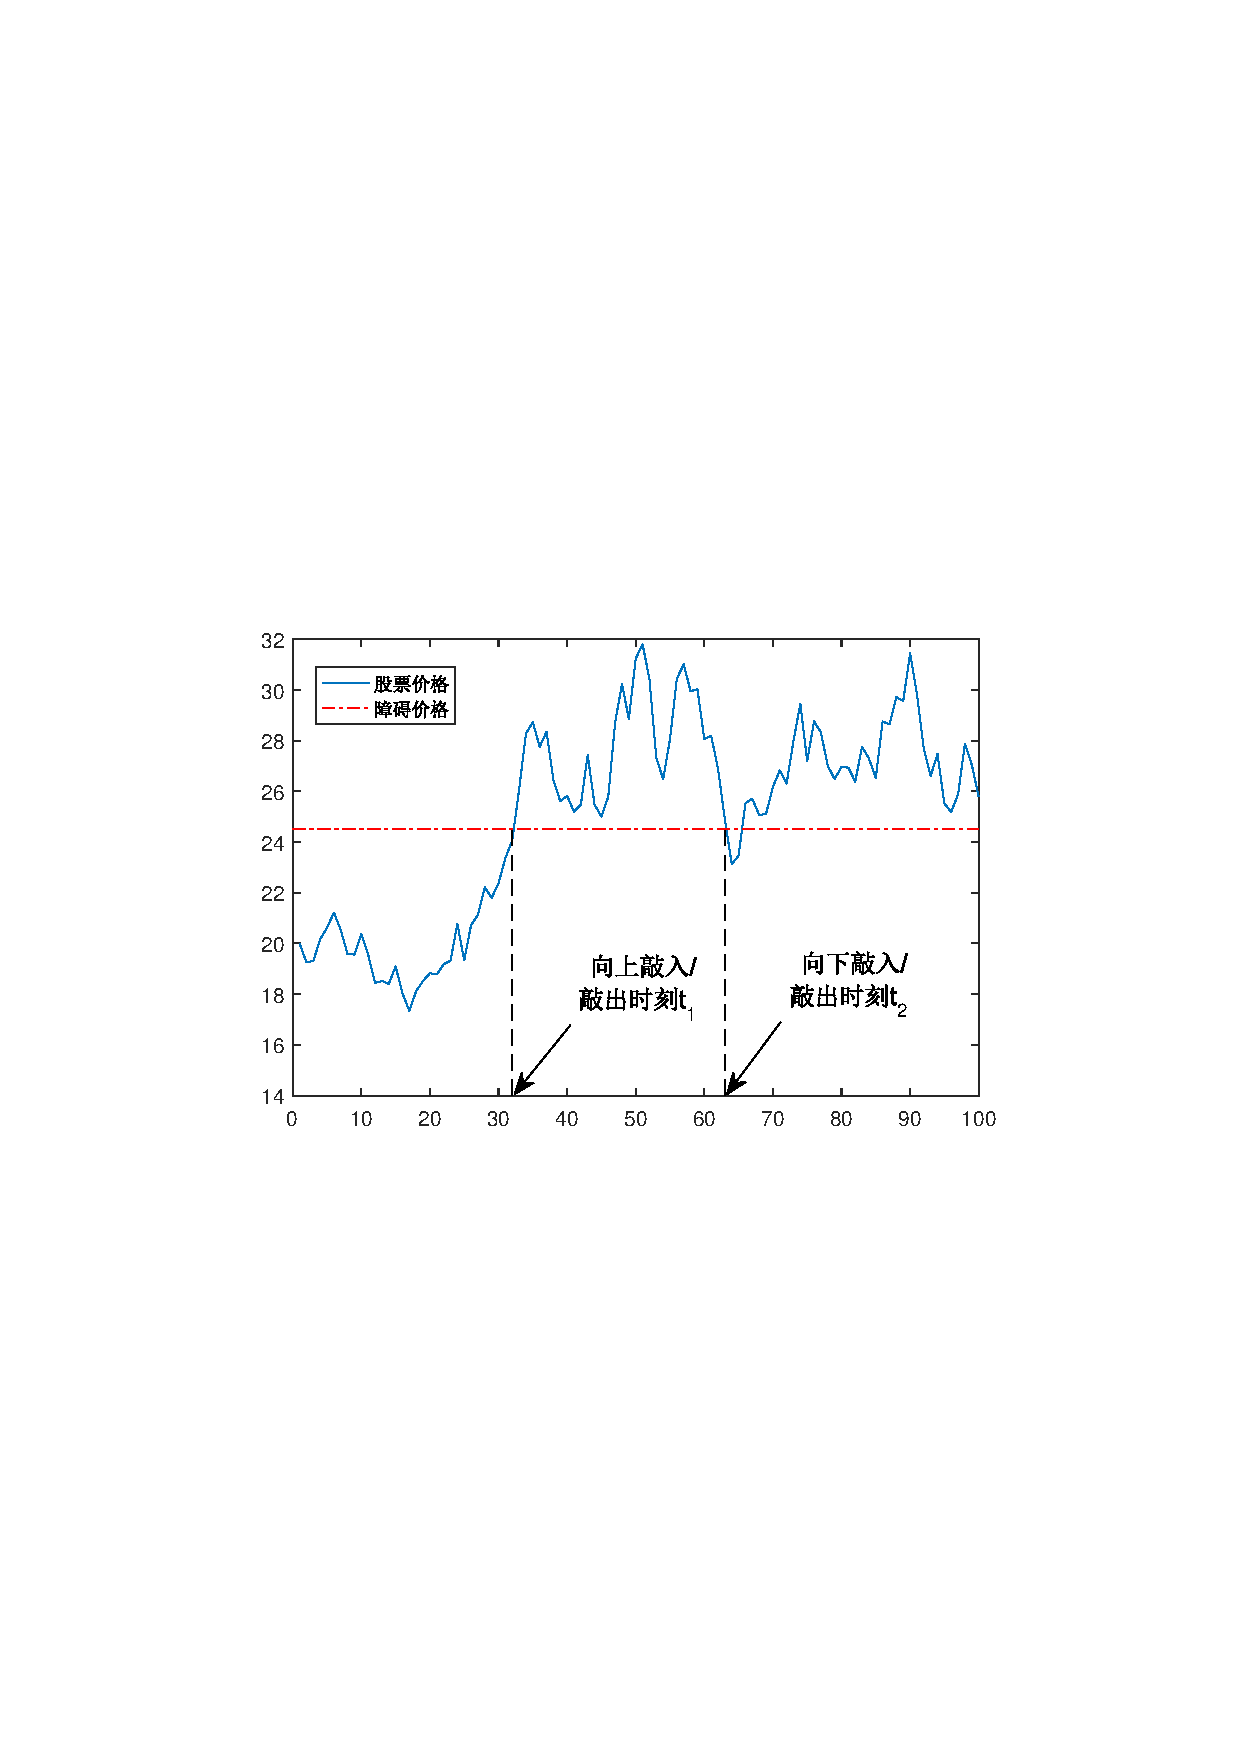
\includegraphics[scale=.8]{fig/barrier2.PDF}
\end{frame}


\begin{frame}{障碍期权的回报函数}\small
	\begin{spacing}{1.3}
	对于障碍期权而言,由于存在一个障碍价格,因此其回报函数要比之前所提及的普通欧式期权和二元期权复杂。对于其中的向上敲入/敲出期权而言,其行权价$K$必须小于障碍价格$B$,否则该期权将一直生效(敲入)或失效(敲出)。对于这类期权而言,其回报函数在形式上需要加入一个示性函数进行判断。比如:对于欧式看涨期权而言,其回报函数如下:
\[\max(S_T-K, 0)=(S_T-K)^+ \]
其中,$S_T$是未来期权到期时刻的标的资产价格,$K$是期权的行权价。但是对于向上敲入欧式看涨期权,其回报函数如下:
\[(S_T-K)^+{\bf 1}_{\{S_t>B\}}=\begin{cases}
(S_T-K)^+,  & S_t>B \\
0, &  S_t\le B
\end{cases},\qquad t\in[0,T] \]
\end{spacing}

\end{frame}

\begin{frame}{障碍期权的回报函数表}
	\centering
	\begin{tabular}{cccc}
		\hline
		类型  & 欧式看涨期权  & 欧式看跌期权 & 约束条件\\
		\hline 
		向上敲入 & $(S_T-K)^+{\bf 1}_{\{S_t>B\}}$ & $(K-S_T)^+{\bf 1}_{\{S_t>B\}}$ &  $K<B$     \\
		向上敲出& $(S_T-K)^+{\bf 1}_{\{S_t<B\}}$ & $(K-S_T)^+{\bf 1}_{\{S_t<B\}}$   &  $K<B$    \\
		向下敲入& $(S_T-K)^+{\bf 1}_{\{S_t<B\}}$ & $(K-S_T)^+{\bf 1}_{\{S_t<B\}}$ &  $K>B$     \\
		向下敲出& $(S_T-K)^+{\bf 1}_{\{S_t>B\}}$ & $(K-S_T)^+{\bf 1}_{\{S_t>B\}}$ &  $K>B$     \\
		\hline
		\end{tabular}
\end{frame}


\begin{frame}{障碍期权定价的基本原理}
	利用风险中性定价法,也可以对障碍期权进行定价。以向上敲入欧式看涨期权为例,其当前时刻的价格$V(0)$可以用条件期望表示如下:
\[V(0)={\rm e}^{-rT}\EQ\left[(S_T-K)^+{\bf 1}_{\{S_t>B\}}|S(0)=S\right] \]
要对上式进行进一步的求解,还需对障碍期权回报函数中的示性函数项进行进一步的化简。根据向上敲入期权的特点可知,一旦在期权有效期之内,标的资产的最高价格超过了障碍价格$B$,该期权就会生效。正因如此,下式必须成立:
\[\{S_t>B\}=\left\{\max_{t\in[0,T]}S_t>B\right\},\qquad \forall t\in[0,T]\]
于是原先的问题就转化成利用$S_t$最大值的概率分布特征求解期权的定价问题。
\end{frame}


\section{B-S模型的不足及拓展}

\subsection{B-S模型的假设条件}

\begin{frame}{B-S模型的假设条件}
	\begin{itemize}
		\item 标的资产价格的变动符合几何布朗运动。相应地,标的资产的价格服从对数正态分布,这保证了标的资产的价格不可能取负值。
		\item 投资者可以无限制卖空标的资产。
		\item 		市场无摩擦,即不存在影响收益的任何外部因素,如税收、交易成本。所有证券都可无限细分。
		\item 		在欧式期权到期前,标的资产无任何收益(如利息、红利等)的支付。于是,标的资产价格的变动是连续的,且是均匀的,既无跳空上涨,也无跳空下跌。
	\end{itemize}
\end{frame}

\begin{frame}{B-S模型的假设条件(cont.)}
			\begin{itemize}
		\item  不存在无风险的套利机会。
		\item 标的资产的交易是连续的,并且标的资产价格波动率是不随时间变化的常数。
		\item 存在一个固定的无风险利率,投资者可以此利率无限制地借贷。
	\end{itemize}
\end{frame}

\subsection{B-S模型的不足和改进}
\begin{frame}{标的资产价格的变动}
	B-S模型当中假设的几何布朗运动虽然保证了资产价格的非负性,但是仍有缺陷,比如:几何布朗运动中,对应的标的资产收益率服从正态分布,这一点与现实金融市场上资产价格尖峰厚尾的特征不相符,盲目使用会极大地低估极端风险;几何布朗运动中,标的资产价格的均值随时间呈现出指数式上升,这一特点与现实市场中利率、大宗商品价格的走势相悖。
\end{frame}


\begin{frame}{标的资产无任何收益的支付}
	对于股票、债券这样的金融资产而言,会存在定期或不定期的收益支付,股票会以股利、送股等方式体现;债券则会以票息的形式给付利息。因此B-S模型自然存在缺陷。以默顿(1973)为代表的学者尝试将股息率(dividend rate)纳入B-S模型当中,从而得到了考虑股息率的B-S-M模型。
\end{frame}


\begin{frame}{固定的无风险利率}
	在金融市场中,利率是影响资产价格变动的重要指标,而B-S模型则假定无风险利率固定不变,这显然与金融市场的现状不符;特别是随着利率衍生品的发展,利率不变的前提条件进一步受到严峻挑战。一些学者开始基于利率期限结构相关理论,为利率类衍生品进行定价。
\end{frame}

\begin{frame}{固定的标的资产波动率}
	金融市场中的资产波动率会随经济周期的变动而发生改变,而在B-S模型中,则是假定标的资产波动率固定不变,这一假设随着“波动率微笑”(volatility smile)现象的发现而受到严重质疑。一些学者开始尝试考虑随机波动率(stochastic volatility, SV)模型。
\end{frame}


\end{document}

